\documentclass[12pt]{article} 
\usepackage[final]{pdfpages}
\usepackage[brazil]{babel} %hifenização em português do brasil
\usepackage[T1]{fontenc} 
\usepackage{ae} %arruma a fonte quando usa o pacote acima
\usepackage[utf8]{inputenc}
\usepackage{graphicx}

\usepackage{hyperref}
\hypersetup{
    colorlinks=false,
    pdfborder={0 0 0},
}
\usepackage{listings}
\usepackage{color}
 
\definecolor{codegreen}{rgb}{0,0.6,0}
\definecolor{codegray}{rgb}{0.5,0.5,0.5}
\definecolor{codepurple}{rgb}{0.58,0,0.82}
\definecolor{backcolour}{rgb}{0.95,0.95,0.92}
 
\lstdefinestyle{mystyle}{
    backgroundcolor=\color{backcolour},   
    commentstyle=\color{codegreen},
    keywordstyle=\color{magenta},
    numberstyle=\tiny\color{codegray},
    stringstyle=\color{codepurple},
    basicstyle=\footnotesize,
    breakatwhitespace=false,         
    breaklines=true,                 
    captionpos=b,                    
    keepspaces=true,                 
    numbers=left,                    
    numbersep=5pt,                  
    showspaces=false,                
    showstringspaces=false,
    showtabs=false,                  
    tabsize=2    
}
 
\lstset{style=mystyle}

\begin{document} % Aqui começa o documento
\begin{center}
\rule{15cm}{0.1pt}

\vspace{1cm}
\begin{huge}
\textbf{Projeto Rock in Rio}
\end{huge}
\vspace{1cm}

\rule{15cm}{0.1pt}

\vspace{1cm}

\textbf{\begin{large}
Dener Cirilo Fontes, João Paulo de Oliveira e \\ Lucas Rossi Rabelo
\end{large}	}

\end{center}
\begin{figure}[!h]
\centering
	
\includegraphics[scale=1.8]{Imagens/transparenteazul03.png}
	\label{Rotul}
\end{figure}
\begin{center}
UNIVERSIDADE FEDERAL DE UBERLÂNDIA

\vspace{0.2cm}




BACHARELADO EM CIÊNCIA DA COMPUTAÇÃO 	

\vspace{0.2cm}


SISTEMAS DE BANCO DE DADOS 				

\vspace{0.2cm}

\thispagestyle{empty}
Maria Camila Nardini Barioni			
\vspace{3cm}

\textbf{\centering 21 de Dezembro \\ \centering 2017}
\end{center}


\tableofcontents %índice
\pagebreak 
\section{Especificação do problema}
O festival de música Rock in Rio ocorre graças a vários patrocínios, na forma de contribuição, proveniente de vários patrocinadores. Os patrocinadores patrocinam um ou mais edições, estas por sua vez ocorrem uma vez por ano, e arrecadam uma certa quantia de dinheiro de acordo com o número de pessoas. Cada edição produz várias mídias, e é necessário guardar seu nome e tipo que as diferenciam, e as mídias produzidas podem ser de vários festivais. Nas edições ocorrem diversas apresentações, e cada uma delas possui sua data e hora de início e término, as apresentações dependem das bandas e palcos, na qual podem ocorrer várias apresentações com uma banda e um palco. Cada banda possui seu nome, que geralmente é único, e o gênero, tendo que várias bandas podem se hospedar em hotéis escolhidos aleatoriamente, para que não ocorra favoritismo entre funcionários e bandas, eles tem seu nome, endereço e telefone. Nas bandas, tocam vários artistas, que devem ter armazenados seus nomes e nacionalidades. Os artistas podem também tocar em mais de uma banda, além de tocarem vários instrumentos, o mesmo instrumento pode ser também tocado por vários artistas, o instrumento deve armazenar seu nome, tipo e número de série.

As bandas também utilizam vários equipamentos disponibilizados pelo festival, e também, os equipamentos podem ser utilizados para várias bandas. Os equipamentos possuem seu número de série que as diferenciam, o Tipo e o Nome do equipamento. O tipo de equipamento pode ser de iluminação, efeito especial, som ou controle.

Nas apresentações, estão envolvidos os palcos, que deve manter seu nome, que é comumente único. Nos palcos trabalham vários funcionários, sendo um único funcionário responsável pelo palco, que podem trabalhar em mais de um palco. Cada funcionário têm seu nome, sexo e CPF, além disso, um funcionário pode ser organizador, assistente de palco, voluntário, que possui uma função ou gerente de palco, que é responsável por um único palco.

\section{Esquema Conceitual}
O esquema conceitual segue no Anexo A.
\subsection{Objetivos}

O banco de dados(BD) visa a modelagem de algumas das edições do Rock in Rio no Brasil, incluindo também os patrocinadores, as mídias produzidas pelos shows do festival, as banda que tocaram no festival, os Hotéis onde ficaram hospedadas e também os Palcos onde ocorreram as apresentações, os equipamento usados nos shows, os instrumentos utilizados, os artistas que contemplaram cada edição, entre outros. Vejamos agora cada componente do BD

\subsection{Patrocinador}

Modelamos de forma que cada patrocinador tenha como atributos:
\begin{itemize}
	\item \textbf{Cod:} Reserva um código que identifica o patrocinador, pois o nome fantasia dos patrocinadores pode;
	\item \textbf{Nome:} Nome fantasia do patrocinador;
\end{itemize}

\subsection{Edição}

Cada patrocinador patrocina(n:m) uma edição. E cada respectiva edição possui:
\begin{itemize}
	\item \textbf{arrecadacao:} A arrecadação que aquela edição conseguiu;
	\item \textbf{Ano:} Ano da edição que a identifica;
	\item \textbf{N\_pessoas:} Número de pessoas que compraram os ingressos para o festival.
\end{itemize}
\subsection{Mídia}

Cada edição do festival produz várias mídias, como CDs, DVDs, Singles, etc. Por outro lado, em algumas mídias incluem gravações de váris festivais (n:m).
\begin{itemize}
\item \textbf{Nome:}  Nome da mídia. È chave primária da mídia
\item \textbf{Tipo:} o tipo da mídia pode ser CD, DVD, etc. É também identificador da mídia
\end{itemize}
\subsection{Apresentação}

A apresentação é uma entidade fraca em relação à banda e palco, pois a existência da apresentação depende da existência dos palcos e das bandas, sendo assim, temos várias apresentações para uma banda e um palco, pois uma banda pode apresentar mais de uma vez no mesmo festival, e também, temos uma banda para cada palco e apresentação e, por fim, há uma banda para cada apresentação\cite{Diego}. Com isso temos o relacionamento apresenta e a entidade apresentação com os atributos:
\begin{itemize}
	\item \textbf{data\_hr\_inicio:} Marca a data/hora do início da apresentação, que é o identificador da apresentação
		\item \textbf{data\_hr\_fim:}  Marca a data/hora do início da apresentação.
\end{itemize}

\subsection{Palco}

Cada Palco possui seu nome e um código que o identifica. Vários funcionários trabalham em vários palcos e cada palco possui um único funcionário como responsável.
	\begin{itemize}
		\item \textbf{Cod:} É o código que identifica o palco em si, ou seja, é a chave primária de palco.
		\item \textbf{Nome:} Nome dos palcos, por exemplo Palco Sunset, Rock Street, Palco Street Dance, etc.
	\end{itemize}
	
\subsection{Funcionário}

Essa Entidade de especialização disjunta possui os tipos de funcionários que trabalham no Rock in Rio. A hierarquia de funcionários com seus atributos fica assim
\cite{elmasri2011sistemas}:

	\begin{enumerate}
		\item Funcionário
		\begin{enumerate}
			\item \textbf{Nome(atribuito):} Nome do funcionário.
			\item \textbf{Sexo(atribuito):} Sexo do funcionário.
			\item \textbf{CPF(atribuito):}  CPF do funcionário que é a chave primária da entidade.
			\item \textbf{Gerente de Palco(especialização):} É responsável por um único palco. Não há gerente sem palco
			\item \textbf{Voluntário(especialização):} Os voluntários são as pessoas que ficarão no festival por conta de manter a segurança durante o festival dependendo de sua função.
				\begin{itemize}
					\item \textbf{Função(atributo):} Descreve a função do voluntário no festival.
				\end{itemize}
			\item \textbf{Assistente de Palco(especialização):} O assistente de palco anuncia a próxima atração e tranquiliza a multidão no caso de atrasos e eventuais imprevistos.
			\item \textbf{Organizador(especialização):} O organizador do festival é a pessoa que organiza o festival inserindo as bandas, verificando horários compatíveis com a edição eu guardando isso no banco
		\end{enumerate}
	\end{enumerate}


\subsection{Banda}

As bandas apresentam nos palcos do festival, e cada banda possui:
\begin{itemize}
\item \textbf{nome:} Nome de cada banda.
\item \textbf{cod:} Identificador da banda.
\item \textbf{Gênero:} Gênero predominante que a banda toca.
\end{itemize}

\subsection{Equipamento}

Cada banda utiliza equipamentos específicos, e cada equipamento têm seu:
\begin{itemize}
\item \textbf{n\_serie:} É o número de série que identifica o equipamento.
\item \textbf{Tipo:} Eles podem ser do tipo efeito especial, iluminação, som ou controle.
\item \textbf{Nome:} Nome do equipamento por exemplo: canhão de luz, mesa de som digital, caixa de som 8000W, etc.
\end{itemize}

\subsection{Hotel}

As bandas precisam ficar nos hotéis conveniados com o Rock in Rio, sendo assim, no MER o hotel possui os atributos:
\begin{itemize}
	\item \textbf{nome:} Nome fantasia do hotel(se houver).
	\item \textbf{endereco:} Mantém o endereço do hotel.
	\item \textbf{telefone:} Além de registrar o telefone do hotel, 		ele também é identificador do hotel
\end{itemize}
\subsection{Artista}

No modelo criado, os artistas tocam na banda e cada um possui:

\begin{itemize}
	\item \textbf{nome:} Nome artístico do artista. Foi decidido colocar esse atributo como chave primária, pois os artistas não repetem nomes no mundo real para poder criar uma personalidade associada à seu nome.
	\item \textbf{nacionalidade:} Nacionalidade do artista.
\end{itemize}
\subsection{Instrumento}

Cada artista que toca em uma banda, toca um instrumento, esse instrumento tem um:
\begin{itemize}
	\item \textbf{nome:} O instrumento tem seu nome. Ele pode ser uma guitarra, flauta, bateria, etc
	\item \textbf{n\_serie:} o Número de série do equipamento o identifica, pois ele é único na fábrica.
	\item \textbf{Tipo:} O tipo do instrumento pode ser de sopro, de cordas, etc.
\end{itemize}

\section{Esquema Relacional}
Segue no anexo B o esquema relacional.
\subsection{Entidades Fortes}
\subsubsection{Patrocinador}
Ficou mapeado assim: \textbf{Patrocinador(\underline{cod}, nome, contribuicao)}

\subsubsection{Edição}
Mapeamos para: \textbf{Edicao(arrecadacao, \underline{ano} , n\_pessoas)}


\subsubsection{Mídia}
Mapeando a chave composta, temos: \textbf{Midia(\underline{nome}, \underline{tipo})}

\subsubsection{Hotel}
Um hotel pode ser diferenciado pelo seu número de telefone, que é único. Assim, temos: \textbf{Hotel (nome, endereço, \underline{telefone})}	

\subsubsection{Banda}
As bandas poderiam ser identificadas por seu nome, mas não há nada que restringe duas bandas com o mesmo nome, então criamos um campo cod para diferencià-las. A chave hotel refere-se ao relacionameno Hospeda-se (1:n) que será abordado adiante. Ficou: \textbf{Banda( \underline{cod}, nome, gênero, hotel(Hotel.cod))}

\subsubsection{Equipamento}
Os equipamentos foram atribuídos um número de série para ser sua chave primária: 
\textbf{Equipamento(nome, tipo, \underline{n\_serie})}

\subsubsection{Instrumento}
Assim como em equipamento, os instrumentos também têm como chave primária um número de série	
\textbf{Instrumento( \underline{n\_serie} , nome\_instrumento, tipo)}

\subsubsection{Artista}
O artista foi mapeado da forma: \textbf{Artista(\underline{nome}, nacionalidade)}

\subsubsection{Palco}
O palco têm a chave estrangeira funcionário para contemplar o relacionamento Responsável, resultando em: \\
\textbf{Palco(nome\_palco, \underline{cod},responsavel(Funcionario.cpf))}

\subsection{Entidade Fraca}

\subsubsection{Apresentação}
A entidade fraca será tratada também mais a frente por participar também de um relacionamento ternário, mas no final o resultado será: \\
\textbf{Apresentacao(\underline{  apresentador(Banda.cod), cod\_palco (Palco.cod), dat\_hr\_inicio}, dat\_hr\_fim, ano(Edição.ano))}

\subsection{Relacionamento 1:1}	
\subsubsection{Responsável}
O responsável, por ser um relacionamento do tipo 1:1 foi adotada a seguinte implementação de mapeamento:\\

\textbf{Palco(nome\_palco, \underline{cod},responsavel(Funcionario.cpf))}\\

Adiante, será citado sobre um gatilho que também auxilia para que o relacionamento se mantenha consistente em 1:1.


\subsection{Relacionamento 1:n}	
	\subsubsection{Hospeda-se}
		Esse relacionamento foi contemplado na relação Banda: \textbf{Banda( \underline{cod}, nome, gênero, hotel(Hotel.cod))}

	\subsubsection{Realizada}
		Já o relacionamento realizada, foi inserido na tabela apresentação: \\ \textbf{Apresentacao(\underline{  apresentador(Banda.cod), cod\_palco (Palco.cod), dat\_hr\_inicio}, dat\_hr\_fim, ano(Edição.ano))}
\subsection{Relacionamento m:n}

\subsubsection{Patrocina}
Utilizando as chaves primárias de patrocinador e edicao, temos: \\
\textbf{Patrocina(\underline{patroc (Patrocinador.cod), edicao (edicao.ano)},contribuicao})

\subsubsection{Produz}
O mapeamento foi feito utilizando as chaves primárias de Mídia 
e a chave de edição:
\textbf{Produz ( \underline{midia (Midia.nome), tipo(Midia.tipo), num\_ed(edicao.ano)})
}
\subsubsection{Utiliza}
O relacionamento Utiliza é o relacionamento m:n de equipamento e banda: 
\textbf{Utiliza( \underline{equipamento (equipamento.n\_serie), banda(Banda.cod)})}

\subsubsection{Toca\_em}
Esse relacionamento contempla em que banda toca cada artista. Um artista pode tocar em uma ou mais bandas em um show, não é comum, mas pode acontecer:
\textbf{Toca\_em (\underline{artista (artista.nome) , banda(banda.cod)})}

\subsubsection{Toca}
Mapeamento de qual artista toca em cada instrumento, ele foi mapeado para uma tabela pois um artista pode tocar mais de um instrumento em um show:\\
\textbf{Toca (\underline{artista(artista.nome), instr (instrumento.n\_serie)})}

\subsubsection{Trabalha}
Esse relacionamento depende do mapeamento de funcionário, que será tratado na seção 3.7. Mas no final, ele ficará assim: \\
\textbf{Trabalha(\underline{palco(Palco.cod), cpf (Funcionario.cpf)})}

\subsection{Relacionamento Ternário}
O relacionamento apresenta, que é ternário, presente no MER, fica contemplado no relacionamento apresentação que contempla a entidade fraca  apresentação, que é fraca em relação a palco e à banda e o relacionamento ternário apresenta ficando da forma:
\textbf{Apresentacao(\underline{  apresentador(Banda.cod), cod\_palco (Palco.cod),} \\ \underline{  dat\_hr\_inicio}, dat\_hr\_fim, ano(Edição.ano))}

\subsection{Especialização}
\subsubsection{Funcionario}
Devido ao baixo número de atributos nas subclasses, a especialização de funcionário foi mapeada da seguinte forma:\\

\textbf{Funcionario(\underline{cpf}, nome, sexo, tipoEmpregado, funcaoVoluntario)}\\

Assim, se um funcionário é voluntário, ele tem sua função, caso contrário a atributo funcao é nulo.
\section{Criação do Banco de Dados}
Segue cada tabela com seu devido código\cite{pg9v1a}:
\subsection{Patrocinador}
Essa tabela foi criada apartir do item 3.1.1 deste material. Definimos um código como chave primária pois dois patrocinadores podem ter o mesmo nome fantasia. A contribuição de um patrocinador tem 2 casa depois da vírgula pois se trata de dinheiro.
\begin{lstlisting}[language=sql]
CREATE TABLE Patrocinador(
	cod					integer,
	nome					varchar(40),
	CONSTRAINT patrocinador_pk PRIMARY KEY (cod)
);

\end{lstlisting}

\subsection{Edição}
A arrecadação do festival é no formato de real, com 2 casa após a vírgula, o ano deve ser depois da primeira edição. O ano foi escolhido como chave primária pois não há 2 edições no mesmo ano. E foi pensada a partir da seção 3.1.2.
\begin{lstlisting}[language=sql]
CREATE TABLE Edicao(
	arrecadacao				numeric(20,2),
	ano					numeric(4,0) CHECK (ano > 0),
	n_pessoas				int CHECK (n_pessoas > 0),
	CONSTRAINT edicao_pk PRIMARY KEY (ano)
);
\end{lstlisting}

\subsection{Mídia}
Cada mídia tem seu nome e  tipo, que pode ser, somente DVD ou CD. Ambas os atributos são chaves primárias, pois pode haver um CD e um DVD com o mesmo nome. E também pode ter vários CDs e vários DVDs. \\

\begin{lstlisting}[language=sql]
CREATE TABLE Midia(
	nome					varchar(40),
	tipo					varchar(10) check(
							tipo = 'DVD' OR
							tipo = 'CD'
						),
	CONSTRAINT midia_pk PRIMARY KEY (nome,tipo)
);
\end{lstlisting}
\subsection{Hotel}
O hotel poder têm 2 atributos que o identificam, que são únicos, que é o telefone e o endereço do hotel. Optou-se por escolher o telefone, pois é uma string menor que implica em uma maior agilidade de execução. Esse trecho foi obtido graças ao item da seção 3.1.4
\begin{lstlisting}[language=sql]
CREATE TABLE Hotel (
	nome					varchar(40),
	endereco				varchar(120),
	telefone				varchar(15),
	CONSTRAINT hotel_pk PRIMARY KEY (telefone)
);
\end{lstlisting}

\subsection{Banda}
Em banda, colocamos um cod serial para que o usuário não se preocupe na hora da inserção, por outro lado, na hora de outra edição ele terá que fazer a busca da banda a ser utilizada na operação. Apesar de não ser comum, as bandas podem ter nomes repetidos. Mas deixamos o nome da banda como chave candidata.
\begin{lstlisting}[language=sql]
CREATE TABLE Banda(
	cod					serial	   ,
	nome					varchar(40),
	genero					varchar(33),
	hotel					varchar(15),
	CONSTRAINT fk_banda FOREIGN KEY (hotel) REFERENCES hotel(telefone),
	CONSTRAINT banda_pk PRIMARY KEY (cod),
	CONSTRAINT generos CHECK (
		UPPER(genero) = 'Heavy Metal' OR 
		UPPER(genero) = 'MPB' OR 
		UPPER(genero) = 'JAZZ' OR 
		UPPER(genero) = 'POP' OR 
		UPPER(genero) = 'ROCK' OR
		UPPER(genero) = 'WORLD'
	)
);
\end{lstlisting}

\subsection{Equipamento}
Na tabela equipamento, há um check para verificar o tipo de equipamento. E também o número de série para diferenciá-lo dos demais.
\begin{lstlisting}[language=sql]
CREATE TABLE Equipamento(
	n_serie					varchar(30),
	nome					varchar(40),
	tipo					varchar(20) 
	CONSTRAINT equipamentos CHECK (
		UPPER(tipo) = 'EFEITO ESPECIAL' OR
		UPPER(tipo) = 'ILUMINACAO' OR
		UPPER(tipo) = 'SOM' OR
		UPPER(tipo) = 'CONTROLE'
	),
	CONSTRAINT equipamento_pk PRIMARY KEY (n_serie)
);
\end{lstlisting}

\subsection{Funcionário}
No caso de voluntário, ele possui uma função. Caso o funcionário não seja voluntário, esse atributo fica com valor \textit{NULL}
\begin{lstlisting}[language=sql]
CREATE TABLE Funcionario(
	cpf						varchar(11),
	nome					varchar(40),
	sexo					char,
	tipoEmpregado			varchar(120),
	funcaoVoluntario		varchar(120),
	CONSTRAINT funcionario_pk	PRIMARY KEY (cpf)
);
\end{lstlisting}

\subsection{Palco}
O código do palco é a chave primária, mas o nome do palco é chave candidata, pois em todas as edições do Rock in Rio, não houve uma edição que teve 2 nomes de palcos iguais.
\begin{lstlisting}[language=sql]
CREATE TABLE Palco(
	nome_palco			varchar(40),
	cod					serial,
	responsavel			varchar(11) NOT NULL,
	CONSTRAINT pk_palco PRIMARY KEY (cod),
	CONSTRAINT fk_palco FOREIGN KEY (responsavel) REFERENCES Funcionario(cpf)
);
\end{lstlisting}

\subsection{Instrumento}
A tabela instrumento guarda as seguintes informações:
\begin{lstlisting}[language=sql]
CREATE TABLE Instrumento(
	n_serie					varchar(30),
	nome_instrumento			varchar(40),
	tipo					varchar(20),
	CONSTRAINT Instrumento_pk PRIMARY KEY (n_serie)
);
\end{lstlisting}
\subsection{Artista}
O artista possui o nome como chave primária, pois nenhum artista possui o mesmo nome artístico.
\begin{lstlisting}[language=sql]
CREATE TABLE Artista(
	nome					varchar(40),
	nacionalidade				varchar(20),
	CONSTRAINT artista_pk PRIMARY KEY (nome)
);
\end{lstlisting}

\subsection{Apresentação}
A apresentação possui um apresentador, que no caso é uma chave estrangeira de banda, uma chave estrangeira de palco. Uma \textit{timestamp} que se refere à data e hora de início da apresentação, além de um ano, que é chave estrangeira de edição. E por fim a data e hora do fim da apresentação.
\begin{lstlisting}[language=sql]
CREATE TABLE Apresentacao(
	apresentador			integer,
	cod_palco 				integer,
	dat_hr_inicio			timestamp,
	dat_hr_fim				timestamp,
	ano 					numeric(4,0) CHECK (ano > 0),
	CONSTRAINT apresentacao_fk  FOREIGN KEY (apresentador) REFERENCES Banda(cod),
	CONSTRAINT apresentacao_fk1 FOREIGN KEY (cod_palco) REFERENCES Palco(cod),
	CONSTRAINT apresentacao_pk  PRIMARY KEY (apresentador,cod_palco,dat_hr_inicio),
	CONSTRAINT ed_fk	    FOREIGN KEY (ano) REFERENCES Edicao(ano)
);
\end{lstlisting}
\subsection{Patrocina}
A tabela patrocina possui chaves estrangeiras referentes às tabelas patrocinador e edição para contemplar o relacionamento patrocina.
\begin{lstlisting}[language=sql]
CREATE TABLE Patrocina(
	patroc					integer,
	edicao					NUMERIC(4,0),
	contribuicao				numeric(10,2) CHECK (contribuicao > 0),
	CONSTRAINT fk_patr	 	FOREIGN KEY (patroc) REFERENCES patrocinador(cod),
	CONSTRAINT fk_edicao		FOREIGN KEY (edicao) REFERENCES edicao(ano),
	CONSTRAINT pk_patrocina 	PRIMARY KEY (patroc,edicao)	
);
\end{lstlisting}

\subsection{Produz}
A tabela produz refere-se ao mapeamento m:n de uma edição que produz várias mídias. Ela possui as chaves estrangeiras que referenciam as chaves primárias de edição e mídia.
\begin{lstlisting}[language=sql]
CREATE TABLE Produz (
	midia					varchar(40),
	tipo					varchar(10),
	ano_ed					NUMERIC(4,0),
	CONSTRAINT fk_edicao FOREIGN KEY (ano_ed) REFERENCES edicao(ano),
	CONSTRAINT fk_tmidia FOREIGN KEY (tipo,midia) REFERENCES midia(tipo,nome),
	CONSTRAINT pk_produz PRIMARY KEY (midia,tipo,ano_ed)
);
\end{lstlisting}

\subsection{Utiliza}
A tabela utiliza refere-se à banda que utiliza certo equipamento, contendo apenas as chaves estrangeiras para contemplar o relacionamento do tipo m:n.
\begin{lstlisting}[language=sql]
CREATE TABLE Utiliza(
	banda					integer,
	equipamento 				varchar(30),
	CONSTRAINT utiliza_pk 	PRIMARY KEY (banda,equipamento),
	CONSTRAINT utiliza_fk	FOREIGN KEY (banda) 		REFERENCES Banda(cod),
	CONSTRAINT utiliza_fk1	FOREIGN KEY (equipamento) 	REFERENCES Equipamento(n_serie)
);
\end{lstlisting}

\subsection{Toca\_em}
Essa tabela refere-se à relação Toca\_em em que um artista toca em uma banda. Ele possui apenas as chaves compatíveis para fazer essa relação válida.
\begin{lstlisting}[language=sql]
CREATE TABLE Toca_em(
	artista 			varchar(40),
	banda				integer,
	CONSTRAINT toca_em_pk 	PRIMARY KEY (artista,banda),
	CONSTRAINT toca_em_fk	FOREIGN KEY (artista) 	REFERENCES Artista(nome),
	CONSTRAINT toca_em_fk1	FOREIGN KEY (banda) 	REFERENCES Banda(cod)
);
\end{lstlisting}

\subsection{Toca}
Essa tabela tem como função mostrar quais artistas tocam quais instrumentos, e mantém a integridade referencial necessária para cumprir tal requisito.
\begin{lstlisting}[language=sql]
CREATE TABLE Toca (
	artista			varchar(40),
	insts 			varchar(30),
	CONSTRAINT toca_pk 	PRIMARY KEY (artista,insts),
	CONSTRAINT toca_fk	FOREIGN KEY (artista) 	REFERENCES Artista(nome),
	CONSTRAINT toca_fk1	FOREIGN KEY (insts) 	REFERENCES instrumento(n_serie)
);
\end{lstlisting}

\subsection{Trabalha}
A tabela trabalha contempla o Funcionário que trabalha em vários palcos.
\begin{lstlisting}[language=sql]
CREATE TABLE Trabalha(
	palco				integer,
	cpf 				varchar(11),
	CONSTRAINT trabalha_pk 	PRIMARY KEY (palco,cpf),
	CONSTRAINT trabalha_fk 	FOREIGN KEY (palco) REFERENCES palco(cod),
	CONSTRAINT trabalha_fk1	FOREIGN KEY (cpf) REFERENCES funcionario(cpf)
);

\end{lstlisting}
\section{Consultas}
\subsection{Número de instrumentos que cada artista toca}
\begin{lstlisting}[language=sql]
SELECT a.nome,COUNT(*) "N de instumentos"
FROM Artista a, Instrumento i, Toca t
WHERE a.nome=t.artista AND i.n_serie=t.insts
GROUP BY a.nome,ARTISTA;
\end{lstlisting}
\subsection{Média de contribuição do festival por edição}
\begin{lstlisting}[language=sql]
SELECT AVG(contribuicao) "Media de contribuicao"
FROM Patrocina p;
\end{lstlisting}

\subsection{Contribuição dos patrocinadores em cada edição do festival em ordem crescente}
\begin{lstlisting}[language=sql]
SELECT edicao , SUM(contribuicao) Patrocinio
FROM PATROCINA, edicao
GROUP BY edicao
ORDER BY edicao asc;

\end{lstlisting}

\subsection{Quais equipamentos foram utilizados pelas bandas que tocaram no palco Sunset}
\begin{lstlisting}[language=sql]
SELECT DISTINCT e.nome
FROM equipamento e, banda b, apresentacao a, palco p, utiliza u
WHERE e.n_serie = u.equipamento AND u.banda=b.cod AND b.cod=a.apresentador AND 
	a.cod_palco = p.cod AND p.nome_palco='Sunset';
\end{lstlisting}


\subsection{Quais funcionários do sexo masculino trabalharam no palco mundo e o nome começa com a letra M}
\begin{lstlisting}[language=sql]
SELECT f.nome
FROM funcionario f, trabalha t, palco p
WHERE f.cpf=t.cpf AND t.palco=p.cod AND f.sexo='M' AND p.nome_palco='Mundo' AND f.nome LIKE 'M%';
\end{lstlisting}

\subsection{Qual Hotel hospeda o maior número de bandas?}
\begin{lstlisting}[language=sql]
SELECT h.nome
FROM hotel h, banda b
WHERE h.telefone = b.hotel
GROUP BY h.nome
HAVING count(*)=(SELECT MAX(cnt)
	FROM (SELECT count(*) cnt
	FROM hotel h, banda b
	WHERE h.telefone = b.hotel
	GROUP BY h.nome) ct);
\end{lstlisting}

\subsection{Qual a média das contribuições feitas pela Sky}
\begin{lstlisting}[language=sql]
SELECT avg(contribuicao)
FROM patrocinador p, patrocina pat
WHERE p.cod = pat.patroc AND p.nome='Sky';
\end{lstlisting}

\subsection{Qual banda tem o menor número de artistas?}
\begin{lstlisting}[language=sql]
SELECT b.nome
FROM banda b, toca_em t, artista a
WHERE b.cod=t.banda AND a.nome=t.artista
GROUP BY b.nome
HAVING count(*)=(SELECT MIN(cnt)
	FROM (SELECT count(*) cnt
	FROM banda b, toca_em t, artista a
	WHERE b.cod=t.banda AND a.nome=t.artista
	GROUP BY b.nome) ct);
\end{lstlisting}

\subsection{Quais bandas apresentaram entre 2013 à 1015?}
\begin{lstlisting}[language=sql]
SELECT b.nome
FROM banda b, apresentacao aP
WHERE b.cod=ap.apresentador AND ap.dat_hr_inicio BETWEEN '2013-01-01 00:00:00' AND '2015-12-31 23:59:00'
GROUP BY B.nome;
\end{lstlisting}

\subsection{Edição e valor do total arrecadado, sendo esse maior que 50000000.00}
\begin{lstlisting}[language=sql]
SELECT edicao, SUM(contribuicao) totalArrecadado
FROM ((SELECT edicao,contribuicao FROM patrocina )UNION(SELECT ano,arrecadacao FROM EDICAO))total
GROUP BY edicao
HAVING SUM(contribuicao) > 50000000.00;
\end{lstlisting}

\subsection{Média de apresentações feitas por festival}
\begin{lstlisting}[language=sql]
SELECT e.ano, avg(apPorAno.count)
FROM Apresentacao ap, edicao e,(SELECT ed.ano, count(*)
		FROM Apresentacao ap, edicao ed
		group by ed.ano) apPorAno
WHERE ap.ano=e.ano
GROUP BY e.ano
\end{lstlisting}

\subsection{Quais funcionários responsáveis pelos palcos nos shows do Foo Fighthers?}
\begin{lstlisting}[language=sql]
SELECT f.nome
FROM banda b, apresentacao ap, palco p,  funcionario f
WHERE b.nome='Foo Fighters' AND b.cod = ap.apresentador AND ap.cod_palco = p.cod AND
	p.responsavel=f.cpf
\end{lstlisting}

\section{Operações de Inserção}
As operações de inserção se encontram no Anexo C.
\section{Gatilhos}
O Banco de dados há 2 gatilhos, que se encontram nas tabelas:
\subsection{Banda}
O gatilho da tabela banda tem como função escolher um hotel aleatoriamente para a banda sendo inserida. Esse \textit{trigger} também tira a possibilidade do atributo ser NULL.
\begin{lstlisting}[language=sql]
CREATE FUNCTION selHotel() RETURNS TRIGGER AS 
$$
DECLARE T HOTEL.telefone%TYPE;
BEGIN
	SELECT telefone INTO T FROM Hotel ORDER BY random() LIMIT 1;
	NEW.Hotel := T;
	
	RETURN 	NEW;
END $$ LANGUAGE 'plpgsql';

CREATE TRIGGER compHotel BEFORE INSERT ON Banda 
FOR EACH ROW EXECUTE PROCEDURE selHotel();
\end{lstlisting}

\subsection{Palco}
O gatilho da tabela palco garante que cada gerente de palco só tenha um palco que ele possa administrar, se o usuário do banco tentar fazer uma inserção ou atualização no banco, esse gatilho fará a verificação: Se o palco tiver mais que um responsável ele trás uma exceção.
\begin{lstlisting}[language=sql]
CREATE OR REPLACE FUNCTION contaResp() RETURNS TRIGGER AS
$$
DECLARE nResp int;
BEGIN
	SELECT COUNT(*) INTO nResp FROM Palco p WHERE p.responsavel = new.responsavel;
	IF nResp = 0 THEN
		RETURN NEW;
	ELSE
		RAISE EXCEPTION 'O funcionario com CPF % ja esta cuidando de um palco',new.responsavel
			USING HINT = 'Selecione outro funcionario para ser gerente do palco';
	END IF;
END $$ LANGUAGE 'plpgsql';

CREATE TRIGGER contaResponsavel BEFORE INSERT OR UPDATE ON Palco
FOR EACH ROW EXECUTE PROCEDURE contaResp();
\end{lstlisting}
\section{Procedimento Armazenado}
O procedimento armazenado consiste em uma função que recebe como entrada um inteiro referente ao ano, que se deseja saber o total da arrecadação até aquele ano. Ou seja, se passado 2010 a função retornará a arrecadação total antes do ano de 2010

\begin{lstlisting}[language=sql]
CREATE OR REPLACE FUNCTION geraReceitaAte(IN anoData int) RETURNS INT AS $$
DECLARE	contrib INT;
DECLARE arrecada INT;
BEGIN
	contrib := 0;
	arrecada  := 0;
	SELECT SUM(contribuicao)
	INTO contrib
	FROM patrocina pat
	WHERE pat.edicao<anoData;

	SELECT SUM(arrecadacao)
	INTO arrecada
	FROM Edicao e
	WHERE e.ano<anoData;
	
	RETURN contrib + arrecada;
END $$ LANGUAGE 'plpgsql';
\end{lstlisting}

\section{Aplicação}

A aplicação em Java contempla 3 tabelas, são elas:
\begin{itemize}
\item Banda
\item Toca\_em
\item Artista
\end{itemize}
Com essas tabelas podemos trabalhar a inserção de novos artistas, novos bandas e inserção de artistas em bandas bem como selecionar o nome e a nacionalidade dos artistas que tocam em uma banda.
A aplicação também contempla as operações de deleção e update nessas três tabelas.
\section{Usuários, grupos e permissões}
Os usuários foram criados para fazer o login na aplicação, portanto, eles só têm permissões sobre as tabelas contempladas na aplicação. Foi criador dois usuários e suas permissões:
\begin{itemize}
	\item \textbf{João:} Pode selecionar os integrantes de uma dada banda.
	\item \textbf{José:} Pode selecionar os integrantes de uma dada banda, inserir, atualizar e deletar qualquer banda, artista e a tabela que relaciona as duas.
\end{itemize}
Segue o código:
\begin{lstlisting}[language=sql]
CREATE ROLE organizador WITH NOSUPERUSER CREATEDB CREATEROLE INHERIT NOLOGIN NOREPLICATION CONNECTION LIMIT -1;  
CREATE ROLE plateia WITH NOSUPERUSER NOCREATEDB NOCREATEROLE INHERIT NOLOGIN NOREPLICATION CONNECTION LIMIT -1;  
GRANT CONNECT ON DATABASE rock_in_rio TO organizador,plateia;
GRANT USAGE ON SCHEMA Palcos TO organizador,plateia;

GRANT SELECT (cod,nome,genero) ON Banda TO plateia;
GRANT SELECT ON Toca_em, Artista,Hotel TO plateia;
REVOKE INSERT, DELETE, UPDATE ON Banda, Toca_em,Artista,Hotel FROM plateia;
GRANT SELECT,INSERT,DELETE,UPDATE ON Banda, Toca_em, Artista, Hotel TO organizador;

GRANT SELECT ON SEQUENCE Banda_cod_seq TO plateia;
GRANT ALL ON SEQUENCE    Banda_cod_seq TO organizador;

CREATE ROLE joao    WITH LOGIN ENCRYPTED PASSWORD '123' ;
CREATE ROLE jose    WITH LOGIN ENCRYPTED PASSWORD '123';

GRANT plateia TO joao;
GRANT organizador TO jose;
\end{lstlisting}
\pagebreak
\appendix
\section{Modelo Entidade Relacionamento}
\begin{figure}[!htb]
 \raggedright
	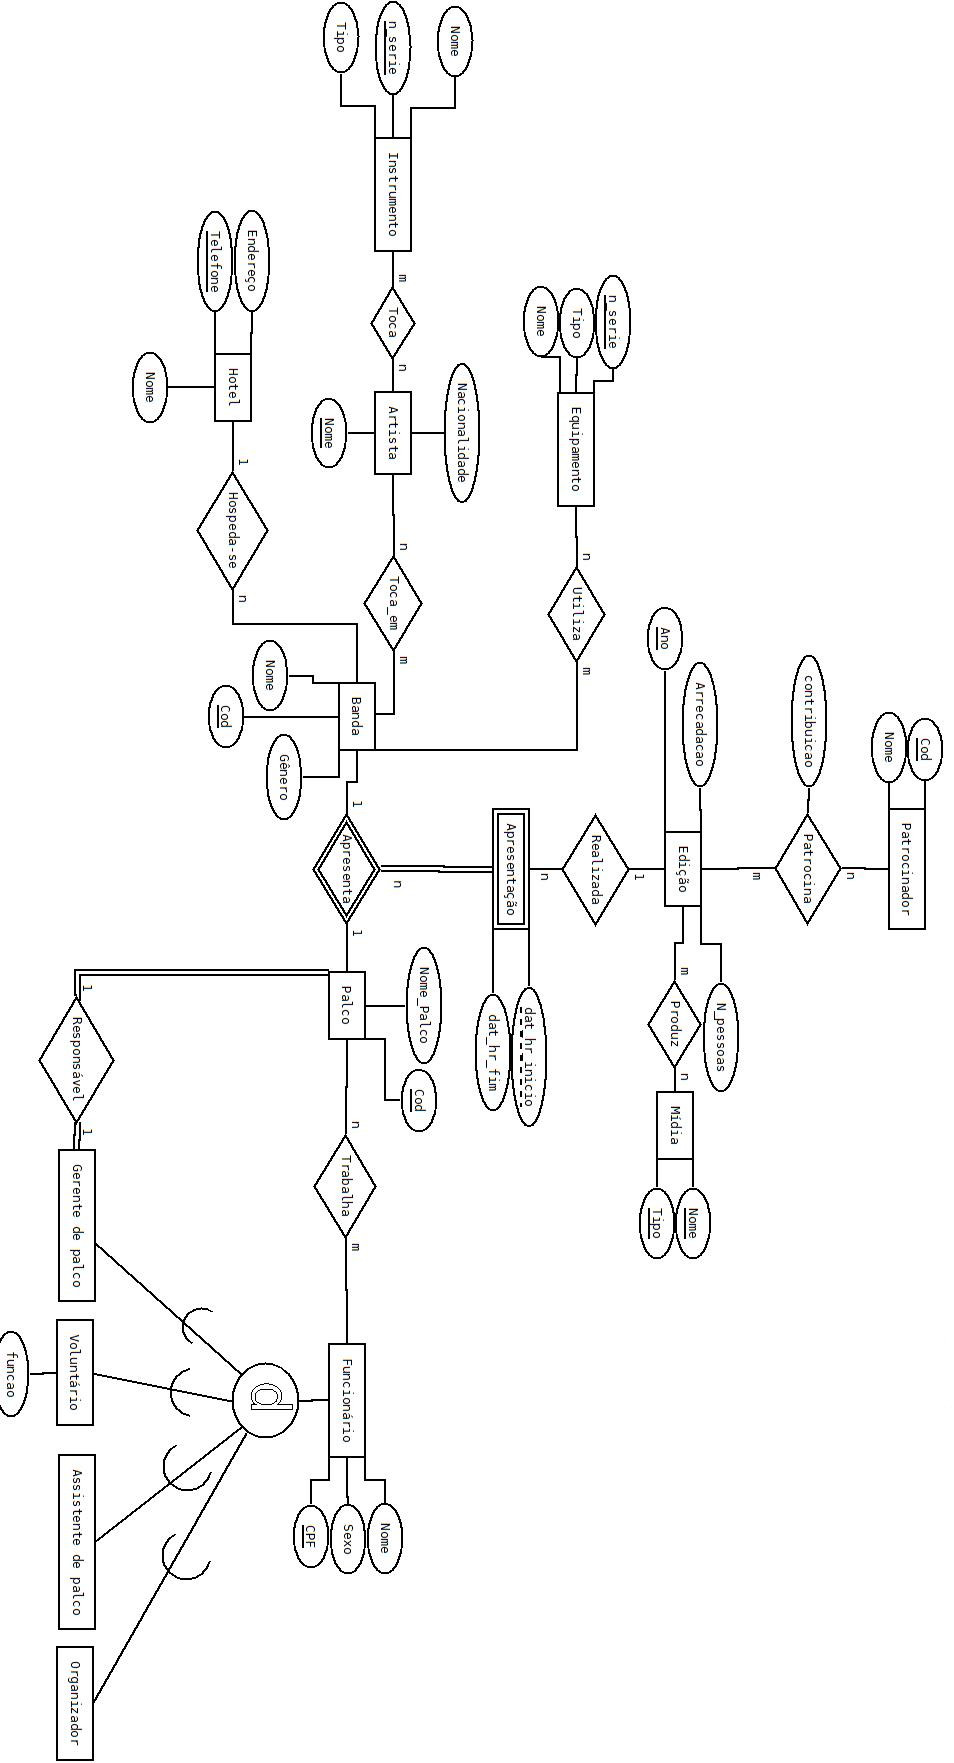
\includegraphics[width=19cm,height=17cm,keepaspectratio]{Imagens/trabfinal.jpeg}
\end{figure}
\pagebreak
%\section{Modelo Relacional}
%\setboolean{@twoside}{false}
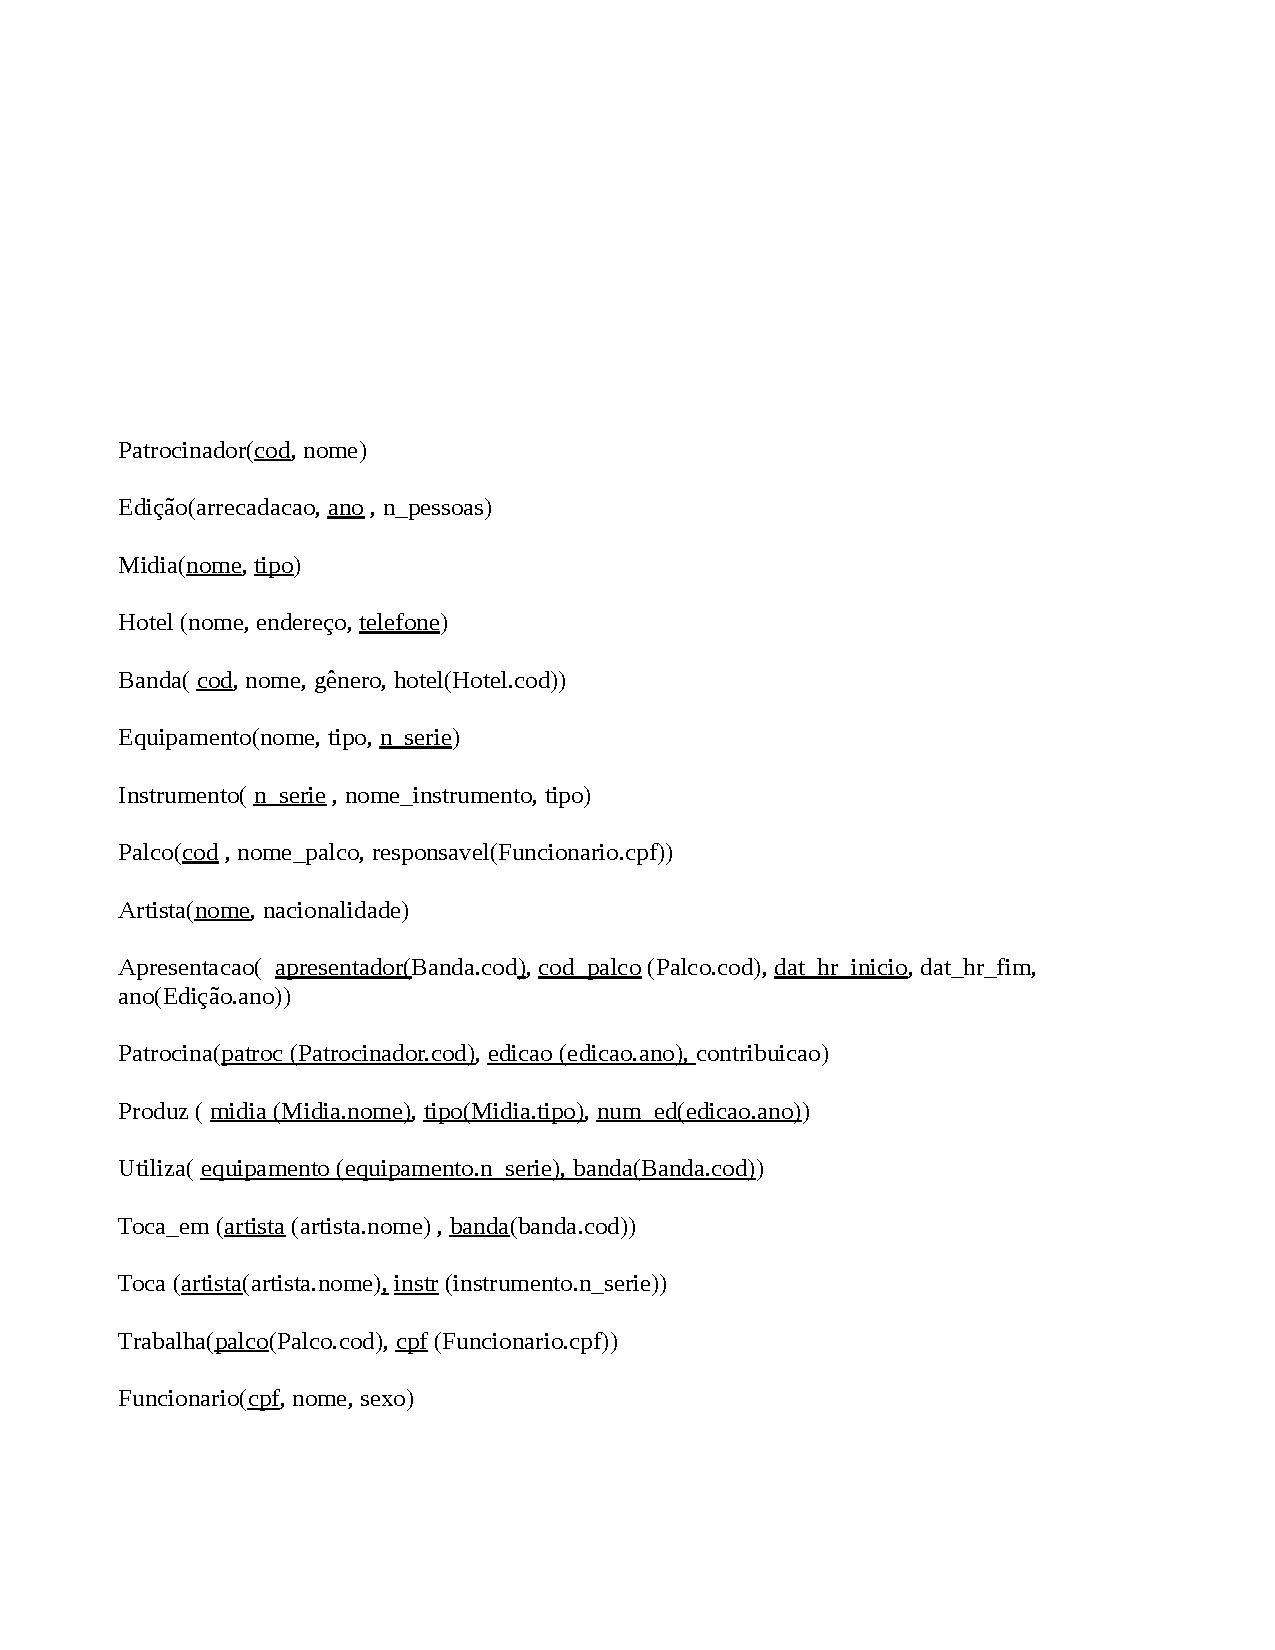
\includepdf[pagecommand={\section{Modelo Relacional} \thispagestyle{empty}}, fitpaper=true]{ModeloRelacional.pdf}
%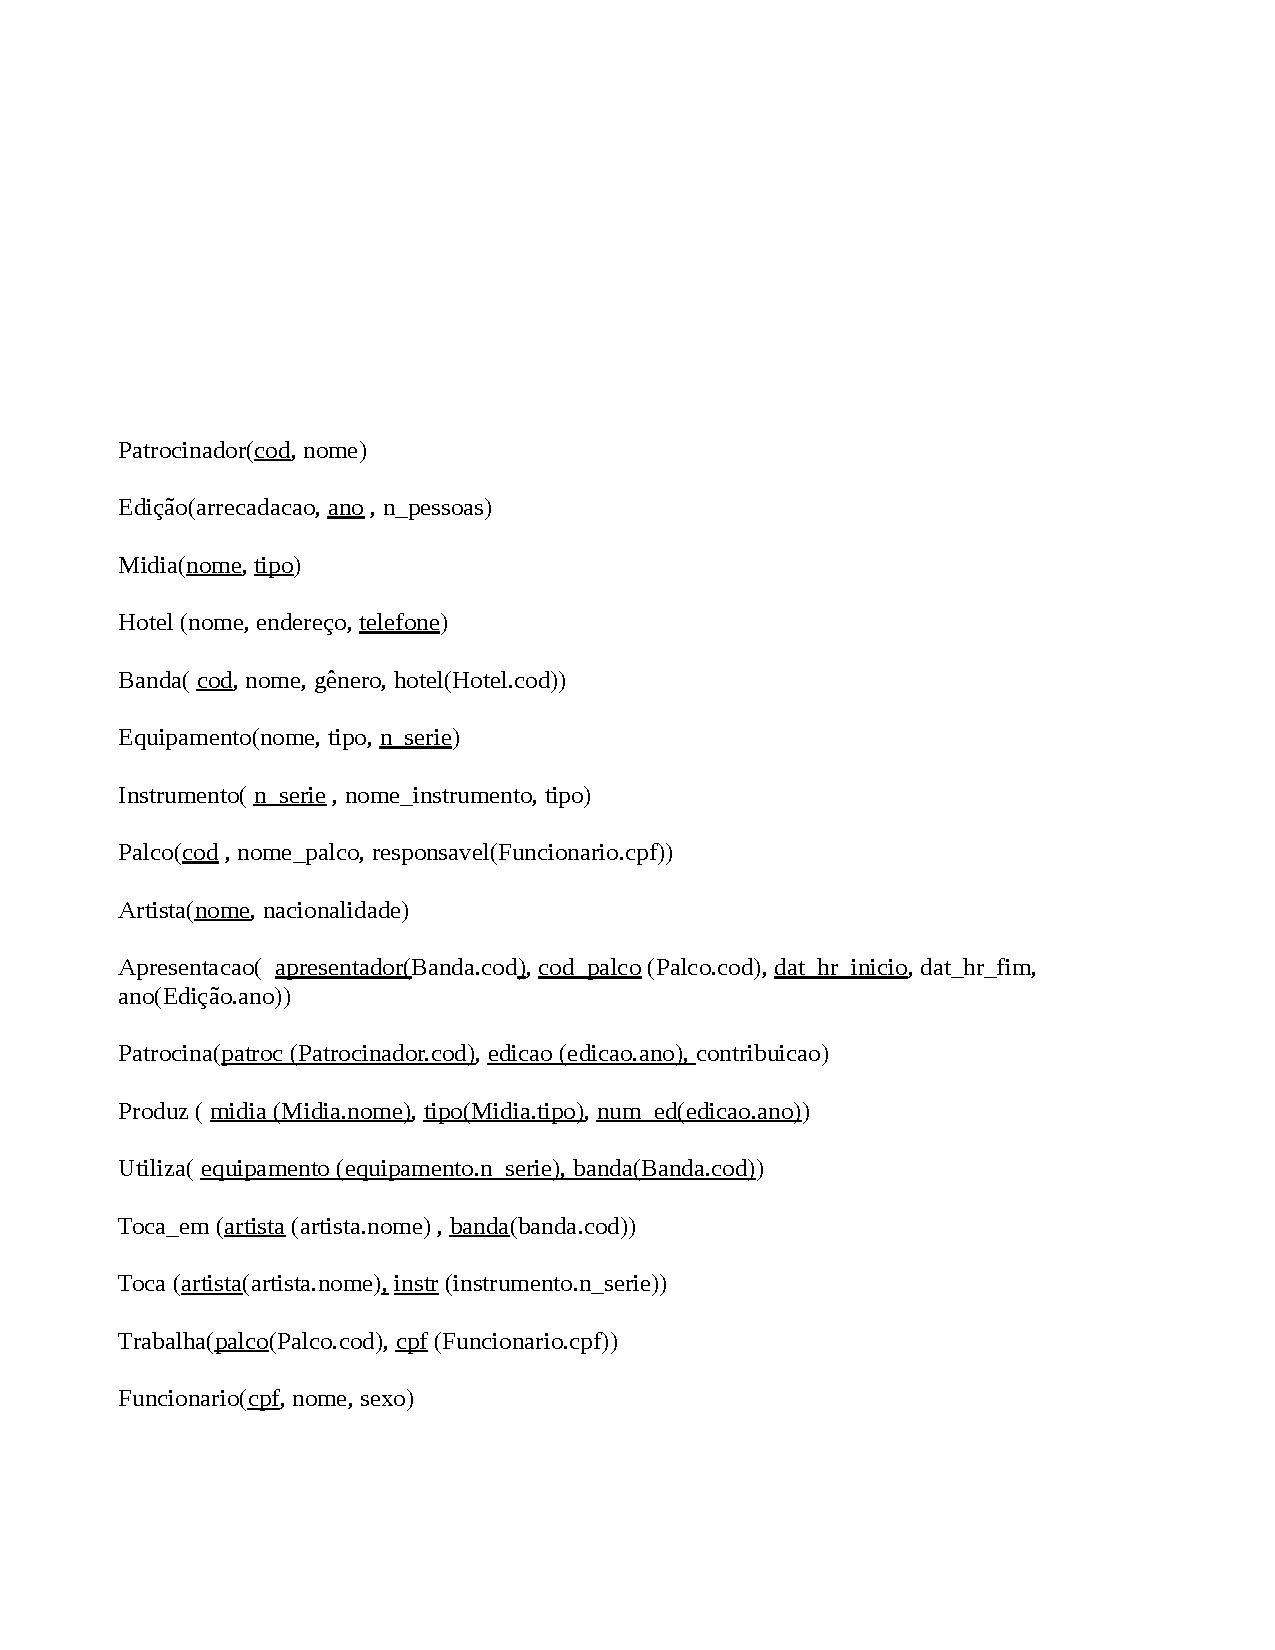
\includepdf[ offset=75 -75, fitpaper=true]{ModeloRelacional.pdf}
\pagebreak
\section{Operações de inserção}
\lstinputlisting [language=sql]{inserts.sql}

\pagebreak
\bibliographystyle{plain}
\bibliography{referencias} 
\end{document}
